\chapter{容错性加强的自动缓存清理模块}\label{chap:clean}

\section{内存管理模块分析}

Spark框架由Scala语言编写。Scala语言是一种运行在JVM(Java Virtual Machine)的函数式编程语言。函数式编程语言相比于C++、Java等命令式编程语言的优点是将数据进行了分类,分为可变数据数据variable和不可变数据value。同时也提供了非常适合并行编程的函数式编程接口。函数式语言的这种特点就让它天然适用于分布式并行大数据处理领域。Scala语言还有一个独特的优势就是它是运行在JVM之上的,这就让Scala语言可以运行在所有支持JVM的平台上,这就使得Scala具有非常好的跨平台特性。但是对于Spark框架来说,他有完全独立的内存管理模块BlockManager。BlockManager也是运行在JVM上的一个进程。

\begin{figure}[htbp]
    \centering
    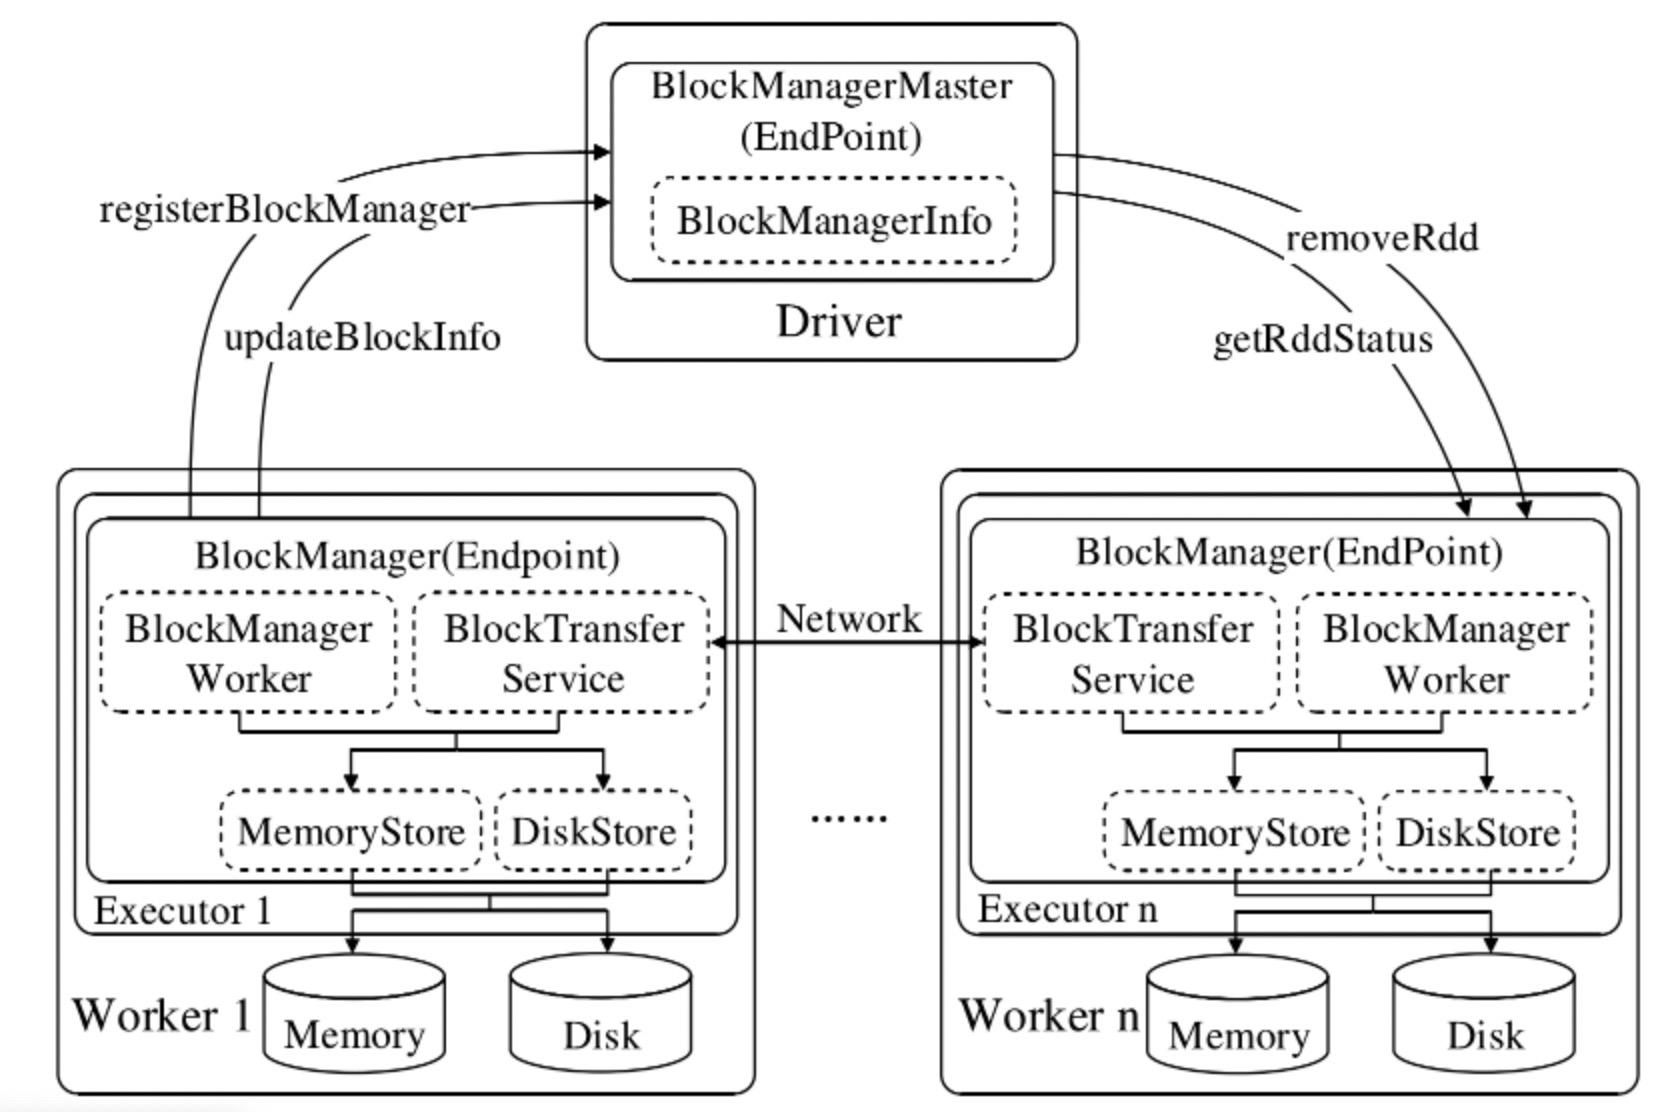
\includegraphics[width=0.99\textwidth]{Img/block-manager.jpg}
    \caption{BlockManager结构图}
    \label{fig:block-manager}
\end{figure}

\subsection{内存管理模块潜在问题}

BlockManager和JVM都有管理内存的功能,但是两者完全隔离,这就会有潜在的问题。BlockManager内存管理的原理非常简单。用户提交Spark应用的时候会通过配置文件指定Executor使用的内存总量,之后框架会向JVM申请内存创建Executor以及内部的BlockManager。BlockManager初始化之后会开始管理Executor整个内存空间。BlockManager向外提供了非常简单的接口,Get接口和Put接口。Get接口的参数为RDD数据的ID,如果数据存储在磁盘或者内存之中BlockManager就会返回具体的地址。Put接口的参数是RDD的应用和存储级别,比如MEMORY\_ONLY、DISK\_ONLY等,BlcokManager会根据存储级别将数据存储在不同位置。

框架的内存模型如图\ref{fig:memory-model}所示。Spark框架内存模型分为以下几个部分:Storage区域,Execution区域,Other区域。Other区域主要用于用户程序定义的数据结构。Execution内存用于框架执行,比如计算RDD的分区时数据就全部存储在Execution区域。Execution区域的内存有一个特点就是会主动地回收内存。他使用的方法是类似与引用计数的算法。比如一个图\ref{fig:simpl-dag}所示的简单的三个节点的计算图。计算得到数据B的时候B的数据就存储在Execution区域。因为计算C还会使用数据B所以数据B并不会立刻被替换出去。但是A会被立刻删除。在以后计算E的时候又会使用到数据A,但是数据A早已被删除,这就会造成数据丢弃,框架会通过容错算法重新计算数据A。

\begin{figure}[htbp]
    \centering
    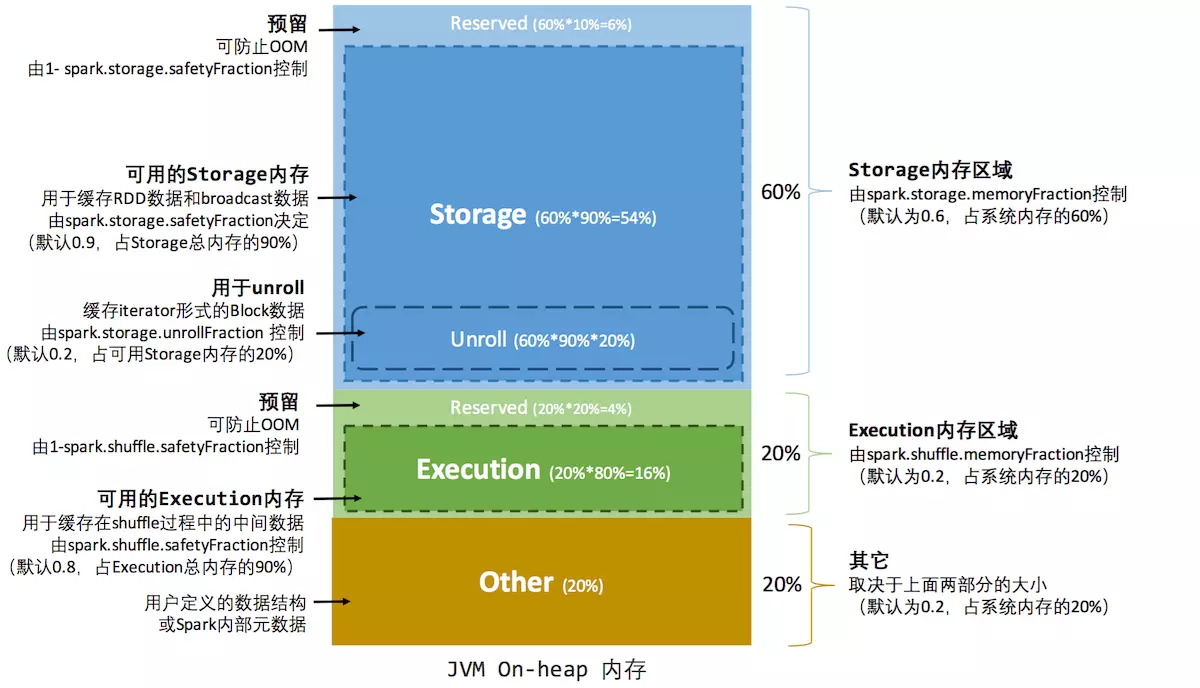
\includegraphics[width=0.99\textwidth]{Img/memory-model.png}
    \caption{内存模型}
    \label{fig:memory-model}
\end{figure}

对于内存管理来说是BlockManager内部的MemoryStore负责的。MemoryStore内部简单地通过一个整数变量记录Executor节点空闲的内存,当收到缓存请求时,MemoryStore会比较空闲空间和需要缓存的数据大小,如果空闲空间大于缓存数据就会保存缓存数据的引用在LinkedHashMap中,这样就能够避免数据被清理。数据放入LinkedHashMap后memoryStore模块会在数值上减少剩余缓存的总量。

通过详细分析Spark框架缓存管理模块的原理可以发现存在着潜在的问题。因为Spark框架的内存管理和JVM虚拟机的内存管理是完全独立的。Spark框架申请内存的行为是一次性的,但是Spark框架释放内存行为和JVM是不同步的。Spark内存管理依赖于JVM的内存回收机制。JVM的自动给回收机制是通过可达性分析实现的。通过从垃圾回收根节点对象出发向下搜索,搜索到的节点为引用链,如果有一些对象没有任何引用链相连,那么这个对象对于内存回收根对象是不可达的,所以将其判定为可回收对象。JVM实际的内存回收原理要复杂得多。根据对内存分析过程的分析可以看到JVM内存回收过程需要进行大量的计算判断,并不能实时地回收内存对象。然而Spark框架的unpersist调用会释放MemoryStore中的RDD对象引用,所以从Spark框架视角看来内存回收立刻就完成了,这就会造成了潜在的风险。对于以下这种场景就有可能超过内存使用上限,造成JVM内存使用超限错误(OOM,Out of Memory error)。具体场景是这样的,Spark应用在执行过程中通过cache调用在内存中缓存了很多RDD数据。缓存空间所剩无几,此时有新的缓存需求,Spark框架就会通过缓存替换策略替换一定数量的数据腾出缓存空间。然而此时JVM内存并没有立刻被回收,但是MemoryStore模块已经认为有了足够的空闲缓存空间,就将新的数据写入缓存空间之中,这就造成了Spark框架使用的内存总量超过了实际向JVM虚拟机申请的总内存,JVM就会杀死Spark框架相关的进程,这就会导致Spark框架奔溃。如图\ref{fig:oom}所示,在第二次内存时因为实际内存并没有释放,就会导致OOM问题。

\begin{figure}[htbp]
    \centering
    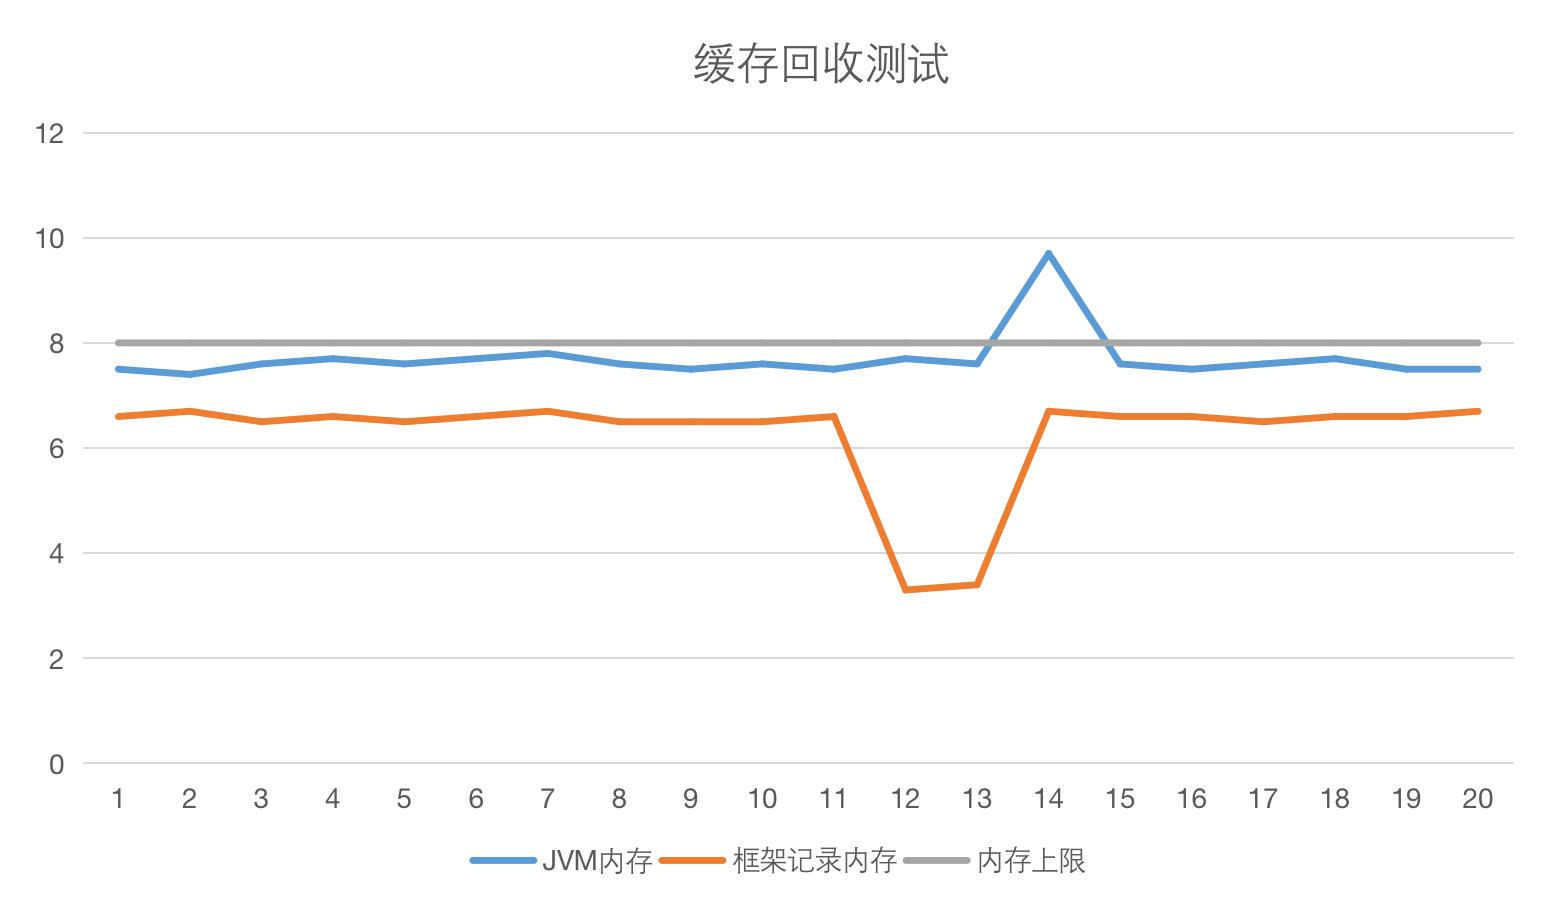
\includegraphics[width=0.99\textwidth]{Img/oom.png}
    \caption{oom问题分析图}
    \label{fig:oom}
\end{figure}


通过分析可以看到Spark框架目前的缓存管理机制是存在着一些潜在的风险的。事实上Spark官方也认识到了这个问题,官方提供的解决方案是设置一个冗余缓冲区,这样就能在一定程度上避免OOM的问题。但是这种解决方案也有一些问题,就是会造成大量内存资源的浪费。

\section{容错性加强的缓存清理模块设计与实现}

\subsection{缓存清理模块设计}

根据对上一节对Spark框架缓存机制的深入分析可以看到目前存在的潜在的问题。官方的解决方法一方面无法完全解决问题,另一方面还会浪费很多内存空间。所以本文从一个新的角度出发来解决这个问题。通过主动清理缓存中的缓存数据,就可以减少减少缓存空间的负载,避免因为负载过高导致内存使用超限的问题。

具体的设计要根据Spark框架的原理来实现,Spark应用提交给Spark框架之后会被解析成一个DAG图执行。通过对DAG图的分析就可以得知什么时候应该清理数据。DAG图中每个点都是RDD数据,DAG图中的边是RDD数据的转换操作。所以对于DAG图中的一个点,它有多少个出边就说明它会在接下来的计算中会被使用多少次。通过对DAG图的分析,就可以得到每个RDD数据在今后计算过程的使用次数n,实际上就是计算节点的出边个数。在计算的过程中,执行一个边的转化操作就将RDD的使用次数减一。这样当RDD的使用次数减为0的时候就说明在正常情况下不会再使用这个RDD数据。此时就可以主动清理MemoryStore模块中的缓存数据。

还有一个问题需要考虑就是作业的容错性。在正常不出错的情况下,在发现RDD数据不会再被使用时就可以清理缓存数据,这种方式可以让缓存空间中的冗余数据最少。然而这种非常激进的缓存清理方式也有它的问题。在出错场景下,Spark框架会根据DAG图的拓扑关系向上游寻找缓存数据,如果找到了缓存数据就可以迅速重新计算丢失的数据,但是如果清理了所有的冗余数据,Spark框架就会从DAG图的输入节点处读取输入数据重新开始计算,这样就会对Spark应用造成巨大的计算延迟。

为了兼顾容错性,可以在清理缓存数据时有选择地保留部分数据。将当前正在计算的RDD数据定义为0,DAG图中每条边的距离为1。具体策略是保存距离正在计算RDD数据小于等于2的数据。这种策略是出于以下考虑,要通过距离为1的RDD数据计算当前RDD数据,所以距离为1的RDD数据肯定需要保存在缓存空间之中。对于距离为2的数据,在计算出错,数据丢失情况下,框架可以通过距离为2的缓存数据迅速重新恢复计算。在小概率场景下距离为2的数据也会丢失,这种小概率场景就只能通过重新计算完成。通过这种设计,通过保留少量冗余数据就可以兼顾系统的容错性。

\subsection{缓存清理模块实现}

这里举一个例子,如图\ref{fig:ft1}所示,黄色节点是正在计算的RDD数据,所有黄色节点的距离为0,黄色RDD节点需要使用距离为1的虚线框中的数据计算得到,所以1号虚框中的数据要保存在内存之中加速计算。在正常计算过程中是只需要使用1号虚框中的数据的,所以灰色节点都可以从缓存中清除出去,从而可以提高缓存空间利用率。然而这种方式的容错性却非常差,在出错场景下会造成严重的重复计算开销。例如图\ref{fig:ft1}所示,红色节点是出错节点,因为在分布式计算数据存在多个机器上,如果某个机器发生问题就会导致这个机器上的数据全部丢失,假设红色节点的数据全部丢失,根据Spark框架的容错原理就需要根据DAG拓扑关系重复计算,具体来说就会计算图\ref{fig:ft1}中红色框中的所有数据,这就会造成大量的重复计算开销。

\begin{figure}[htbp]
    \centering
    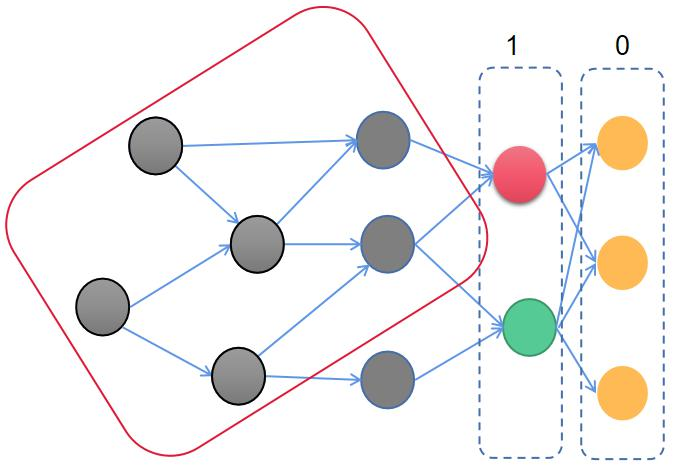
\includegraphics[width=0.6\textwidth]{Img/ft1.png}
    \caption{出错场景重复计算问题}
    \label{fig:ft1}
\end{figure}

本文的容错性加强策略就可以兼顾缓存空间使用效率和容错性。如图\ref{fig:ft2}所示,同样黄色节点是正在计算的节点,同样需要使用1号虚框中的数据计算黄色节点。2号虚框中的数据是距离黄色虚框中所有节点距离为2个节点。通过将2号虚框中的蓝色节点也都保留在内存之中,就可以在出错场景下快速恢复计算。同样红色节点是出错节点,在出错场景下同样会根据容错机制根据DAG图重复计算,但是因为2号虚框中的数据都缓存在内存之中,框架只需要重复计算图\ref{fig:ft2}中红色框中的数据就可以快速恢复计算。可见相比于\ref{fig:ft1},本文的设计能够极大的减少出错场景下重复计算量,从而极大增加了系统的容错性。同时也兼顾了内存资源的使用效率。算法\ref{alg:cal-dis}会返回一个需要清理的rdd列表,之后调用unpersist接口清理所有的缓存数据即可。

\begin{figure}[htbp]
    \centering
    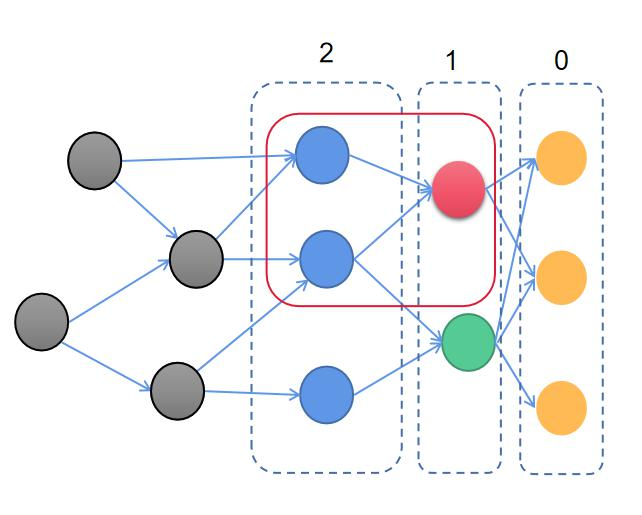
\includegraphics[width=0.6\textwidth]{Img/ft2.png}
    \caption{出错场景快速恢复}
    \label{fig:ft2}
\end{figure}

\begin{algorithm}  
    \caption{缓存清理算法}  
    \begin{algorithmic}[1] %每行显示行号  
        \Require 正在计算的RDD节点列表
        \Ensure 需要清理的数据节点
        \Function{CLEAN\_CACHE}{$ARRAY<RDD> \ rdds$}
            \State $queue \gets \ new \ Queue()$
            \State $dis \gets  \ new \ HashMap()$
            \State $cleanRdds \gets \ new \ Array()$
            \For{$rdd \in rdds$}
                \State $queue.enqueue(rdd)$
                \State $dis[rdd] \gets 0$
            \EndFor
            \While{$!queue.isEmpty()$}
                \State $rdd \gets queue.pop()$
                \State $predecessors \gets rdd.getPredecessors()$
                \For{$predecessor \in predecessors$}
                    \State $queue.enqueue(predecessor)$
                    \State $dis[predecessor] \gets dis[rdd]+1$
                    \If{$dis[predecessor] > 2 \ AND \ predecessor.SRORAGE\_LEVEL == MEMORY\_ONLY$}
                        $cleanRdds.append(predecessor)$
                    \EndIf
                \EndFor
            \EndWhile
        \EndFunction
    \end{algorithmic}
    \label{alg:cal-dis}
\end{algorithm}

\section{实验测试与分析}
\section{本章总结}
